%==============================================================================
% MATH 110 - Section 1A Notes: R^n and C^n
% Linear Algebra Done Right, 4th ed. - Sheldon Axler
%==============================================================================

\documentclass[10pt, twocolumn]{article}
\usepackage[margin=0.75in, columnsep=0.3in]{geometry}

%------------------------------------------------------------------------------
% PACKAGES
%------------------------------------------------------------------------------
\usepackage{amsmath, amssymb, amsthm}
\usepackage{enumitem}
\usepackage{fancyhdr}
\usepackage{titlesec}
\usepackage{tcolorbox}
\tcbuselibrary{breakable}
\usepackage{booktabs}
\usepackage{tikz}
\usetikzlibrary{matrix, arrows.meta, positioning, calc, cd, shapes.geometric}
\usepackage{graphicx}

% TikZ style definitions for consistent diagrams
\tikzset{
    vector/.style={->, >=Stealth, thick},
    axis/.style={->, thin},
    point/.style={fill, circle, inner sep=1.5pt}
}

%------------------------------------------------------------------------------
% SPACING
%------------------------------------------------------------------------------
\linespread{1.08}
\setlength{\parskip}{0.4ex plus 0.2ex minus 0.1ex}

%------------------------------------------------------------------------------
% BOX STYLES
%------------------------------------------------------------------------------
\tcbset{
    boxrule=0.8pt,
    colback=white,
    colframe=black,
    arc=0pt,
    boxsep=3pt,
    left=4pt, right=4pt, top=4pt, bottom=4pt,
    breakable
}

\newtcolorbox{result}{
    boxrule=0pt,
    colback=black!5,
    colframe=white,
    arc=0pt,
    boxsep=2pt,
    left=4pt, right=4pt, top=4pt, bottom=4pt,
    breakable
}

%------------------------------------------------------------------------------
% SECTION FORMATTING
%------------------------------------------------------------------------------
\titleformat{\section}{\large\bfseries}{\thesection.}{0.5em}{}
\titleformat{\subsection}{\normalsize\bfseries}{\thesubsection}{0.5em}{}
\titlespacing*{\section}{0pt}{1.5ex}{1ex}
\titlespacing*{\subsection}{0pt}{1ex}{0.5ex}

%------------------------------------------------------------------------------
% LIST FORMATTING
%------------------------------------------------------------------------------
\setlist{itemsep=1pt, topsep=3pt, parsep=1pt, leftmargin=1.5em}

%------------------------------------------------------------------------------
% HEADER/FOOTER
%------------------------------------------------------------------------------
\pagestyle{fancy}
\fancyhf{}
\fancyhead[L]{\small MATH 110}
\fancyhead[R]{\small Section 1A}
\fancyfoot[C]{\small\thepage}
\renewcommand{\headrulewidth}{0.4pt}

%------------------------------------------------------------------------------
% THEOREM ENVIRONMENTS
%------------------------------------------------------------------------------
\theoremstyle{definition}
\newtheorem{property}{Property}
\newtheorem{definition}{Definition}
\newtheorem{example}{Example}

\theoremstyle{plain}
\newtheorem{theorem}{Theorem}
\newtheorem{lemma}{Lemma}
\newtheorem{proposition}{Proposition}
\newtheorem{corollary}{Corollary}

%------------------------------------------------------------------------------
% CUSTOM COMMANDS
%------------------------------------------------------------------------------
% Number fields
\newcommand{\R}{\mathbb{R}}
\newcommand{\C}{\mathbb{C}}
\newcommand{\F}{\mathbb{F}}
\newcommand{\Z}{\mathbb{Z}}
\newcommand{\Q}{\mathbb{Q}}

% Matrix/space operations
\DeclareMathOperator{\rank}{rank}
\DeclareMathOperator{\nullity}{nullity}
\DeclareMathOperator{\tr}{tr}
\DeclareMathOperator{\spn}{span}
\DeclareMathOperator{\col}{col}
\DeclareMathOperator{\row}{row}
\DeclareMathOperator{\nul}{null}
\DeclareMathOperator{\range}{range}
\DeclareMathOperator{\im}{im}

% Inner products and norms
\newcommand{\inner}[2]{\langle #1, #2 \rangle}
\newcommand{\norm}[1]{\| #1 \|}
\newcommand{\proj}{\operatorname{proj}}

% Vectors and matrices
\newcommand{\vect}[1]{\mathbf{#1}}
\newcommand{\mat}[1]{\mathbf{#1}}

%==============================================================================
\begin{document}
%==============================================================================

\noindent
\begin{minipage}{\linewidth}
    \centering
    \textbf{\Large Section 1A: $\R^n$ and $\C^n$} \\[0.5em]
    \hrule
\end{minipage}
\vspace{1em}

%==============================================================================
\section{Complex Numbers}
%==============================================================================

Before we can study vector spaces, we need to understand the scalars we'll use. The real numbers $\R$ are familiar, but linear algebra becomes more powerful when we also work with complex numbers $\C$.

\begin{tcolorbox}
\textbf{1.1 Definition: Complex Numbers, $\C$}

\begin{itemize}
    \item A \textbf{complex number} is an ordered pair $(a, b)$ where $a, b \in \R$, written as $a + bi$.
    \item The set of all complex numbers is denoted by $\C$:
    \[
        \C = \{a + bi : a, b \in \R\}
    \]
    \item \textbf{Addition} and \textbf{multiplication} on $\C$ are defined by:
    \begin{align*}
        (a + bi) + (c + di) &= (a + c) + (b + d)i \\
        (a + bi)(c + di) &= (ac - bd) + (ad + bc)i
    \end{align*}
    where $a, b, c, d \in \R$.
\end{itemize}
\end{tcolorbox}

\textbf{Intuition:} Think of $\C$ as a 2D plane where the horizontal axis represents real numbers and the vertical axis represents imaginary numbers. If $a \in \R$, we identify $a + 0i$ with the real number $a$, so $\R \subset \C$. We write $0 + bi$ as just $bi$, and $0 + 1i$ as just $i$.

\textbf{Why complex numbers?} Even when working with real matrices, eigenvalues (Chapter 5) often require complex numbers. The completeness of $\C$ makes linear algebra more elegant---every polynomial has roots in $\C$.

\textbf{Why this multiplication formula?} We \textit{define} $i$ as a symbol satisfying $i^2 = -1$. This is consistent and creates an algebraically closed field. Using the usual rules of arithmetic:
\begin{align*}
    (a + bi)(c + di) &= ac + adi + bci + bdi^2 \\
    &= ac + adi + bci - bd \\
    &= (ac - bd) + (ad + bc)i
\end{align*}

\begin{tcolorbox}[colframe=black!50]
\textbf{1.2 Example: Complex Arithmetic}

Compute $(2 + 3i)(4 + 5i)$.

Using the distributive and commutative properties:
\begin{align*}
    (2 + 3i)(4 + 5i) &= 2 \cdot (4 + 5i) + (3i)(4 + 5i) \\
    &= 2 \cdot 4 + 2 \cdot 5i + 3i \cdot 4 + (3i)(5i) \\
    &= 8 + 10i + 12i - 15 \\
    &= \boxed{-7 + 22i}
\end{align*}
\end{tcolorbox}

\begin{tcolorbox}
\textbf{1.3 Properties of Complex Arithmetic}

For all $\alpha, \beta, \lambda \in \C$:

\textbf{commutativity:} $\alpha + \beta = \beta + \alpha$ and $\alpha\beta = \beta\alpha$

\textbf{associativity:} $(\alpha + \beta) + \lambda = \alpha + (\beta + \lambda)$ and $(\alpha\beta)\lambda = \alpha(\beta\lambda)$

\textbf{identities:} $\lambda + 0 = \lambda$ and $\lambda \cdot 1 = \lambda$

\textbf{additive inverse:} For every $\alpha \in \C$, there exists a unique $\beta \in \C$ such that $\alpha + \beta = 0$

\textbf{multiplicative inverse:} For every $\alpha \in \C$ with $\alpha \neq 0$, there exists a unique $\beta \in \C$ such that $\alpha\beta = 1$

\textbf{distributive property:} $\lambda(\alpha + \beta) = \lambda\alpha + \lambda\beta$
\end{tcolorbox}

\begin{tcolorbox}[colframe=black!50]
\textbf{1.4 Example: Commutativity of Complex Multiplication}

To show $\alpha\beta = \beta\alpha$ for all $\alpha, \beta \in \C$, suppose $\alpha = a + bi$ and $\beta = c + di$ where $a, b, c, d \in \R$.

\textbf{LHS:}
\[
    \alpha\beta = (a + bi)(c + di) = (ac - bd) + (ad + bc)i
\]

\textbf{RHS:}
\[
    \beta\alpha = (c + di)(a + bi) = (ca - db) + (cb + da)i
\]

Since real multiplication is commutative ($ac = ca$, $bd = db$, etc.), we have $\alpha\beta = \beta\alpha$. \hfill $\square$
\end{tcolorbox}

\begin{tcolorbox}
\textbf{1.5 Definition: $-\alpha$, Subtraction, $1/\alpha$, Division}

Suppose $\alpha, \beta \in \C$.
\begin{itemize}
    \item Let $-\alpha$ denote the \textbf{additive inverse} of $\alpha$: the unique complex number such that $\alpha + (-\alpha) = 0$.
    \item \textbf{Subtraction} on $\C$ is defined by $\beta - \alpha = \beta + (-\alpha)$.
    \item For $\alpha \neq 0$, let $1/\alpha$ and $\frac{1}{\alpha}$ denote the \textbf{multiplicative inverse} of $\alpha$: the unique complex number such that $\alpha(1/\alpha) = 1$.
    \item For $\alpha \neq 0$, \textbf{division} by $\alpha$ is defined by $\beta/\alpha = \beta(1/\alpha)$.
\end{itemize}
\end{tcolorbox}

\textbf{Computing $1/\alpha$:} For $\alpha = a + bi \neq 0$, multiply by the conjugate:
\begin{result}
\[
    \frac{1}{a + bi} = \frac{a - bi}{a^2 + b^2} = \frac{a}{a^2 + b^2} - \frac{b}{a^2 + b^2}i
\]
\end{result}

\textbf{Key insight:} Why multiply by the conjugate? Because $(a + bi)(a - bi) = a^2 + b^2$ is always real and positive. Multiplying by the conjugate eliminates $i$ from the denominator.

\textbf{Example: Complex Division.} Compute $\displaystyle\frac{2+3i}{4+5i}$.

Multiply by the conjugate of the denominator:
\[
    \frac{2+3i}{4+5i} \cdot \frac{4-5i}{4-5i} = \frac{(2+3i)(4-5i)}{(4+5i)(4-5i)}
\]

Denominator: $(4+5i)(4-5i) = 16 + 25 = 41$

Numerator: $(2+3i)(4-5i) = 8 - 10i + 12i + 15 = 23 + 2i$

\textbf{Answer:} $\displaystyle\frac{2+3i}{4+5i} = \boxed{\frac{23}{41} + \frac{2}{41}i}$

\begin{tcolorbox}
\textbf{1.6 Notation: $\F$}

Throughout this book, $\F$ stands for either $\R$ or $\C$.
\end{tcolorbox}

\textbf{Why use $\F$?} The letter $\F$ reminds us of ``field.'' Both $\R$ and $\C$ are fields: sets with addition and multiplication satisfying the properties in 1.3. Using $\F$ lets us state theorems once and have them apply to both $\R$ and $\C$.

Elements of $\F$ are called \textbf{scalars}.

\textbf{Powers of scalars:} For $\alpha \in \F$ and a positive integer $m$:
\begin{result}
\[
    \alpha^m = \underbrace{\alpha \cdot \alpha \cdots \alpha}_{m \text{ times}}
\]
\end{result}

This definition implies:
\begin{itemize}
    \item $(\alpha^m)^n = \alpha^{mn}$
    \item $(\alpha\beta)^m = \alpha^m \beta^m$
\end{itemize}

%==============================================================================
\newpage
\section{Lists}
%==============================================================================

To generalize $\R^2$ and $\R^3$ to higher dimensions, we first need to discuss the concept of lists.

\begin{tcolorbox}[colframe=black!50]
\textbf{1.7 Example: $\R^2$ and $\R^3$}
\begin{itemize}
    \item $\R^2 = \{(x,y) : x, y \in \R\}$ (the plane)
    \item $\R^3 = \{(x,y,z) : x, y, z \in \R\}$ (3D space)
\end{itemize}
\end{tcolorbox}

\begin{tcolorbox}
\textbf{1.8 Definition: List, Length}

Suppose $n$ is a nonnegative integer. A \textbf{list} of \textbf{length} $n$ is an ordered collection of $n$ elements (which might be numbers, other lists, or more abstract objects) separated by commas and surrounded by parentheses.

A list of length $n$ is also called an \textbf{$n$-tuple}.
\end{tcolorbox}

\textbf{Key point:} Two lists are equal if and only if they have the same length and the same elements in the same order.

\begin{tcolorbox}[colframe=black!50]
\textbf{1.9 Example: Lists versus Sets}
\begin{itemize}
    \item Lists $(3,5)$ and $(5,3)$ are \textbf{not equal}, but sets $\{3,5\} = \{5,3\}$
    \item Lists $(4,4)$ and $(4,4,4)$ are \textbf{not equal}, but sets $\{4,4\} = \{4,4,4\} = \{4\}$
\end{itemize}
Key difference: order and repetition matter in lists, not in sets.
\end{tcolorbox}

\textbf{Why lists?} Linear algebra needs ordered data. The coordinates $(1,2,3)$ represent a different point than $(3,2,1)$. Order encodes meaning---the first coordinate might be position, the second velocity, the third acceleration.

%==============================================================================
\section{$\F^n$}
%==============================================================================

To define the higher-dimensional analogues of $\R^2$ and $\R^3$, we simply replace $\R$ with $\F$ (which equals $\R$ or $\C$) and replace the 2 or 3 with an arbitrary positive integer.

\begin{tcolorbox}
\textbf{1.10 Notation: $n$}

Fix a positive integer $n$ for the rest of this chapter.
\end{tcolorbox}

\begin{tcolorbox}
\textbf{1.11 Definition: $\F^n$}

$\F^n$ is the set of all lists of length $n$ of elements of $\F$:
\[
    \F^n = \{(x_1, x_2, \ldots, x_n) : x_k \in \F \text{ for } k = 1, \ldots, n\}
\]

For $(x_1, \ldots, x_n) \in \F^n$ and $k \in \{1, \ldots, n\}$, we say $x_k$ is the $k^{\text{th}}$ \textbf{coordinate} of $(x_1, \ldots, x_n)$.
\end{tcolorbox}

\begin{example}[Elements of $\F^n$]
\begin{itemize}
    \item $(2, -1, 5) \in \R^3$ is a list with 3 real coordinates.
    \item $(1+i, 2, -3i) \in \C^3$ is a list with 3 complex coordinates.
    \item $(7, -2) \in \R^2$ corresponds to a point in the plane.
    \item $\F^1$ can be identified with $\F$.
\end{itemize}
\end{example}

\textbf{Intuition:} Think of $\R^2$ as the plane and $\R^3$ as 3-dimensional space. For $n > 3$, we lose geometric visualization but the algebra works identically.

\smallskip
\begin{center}
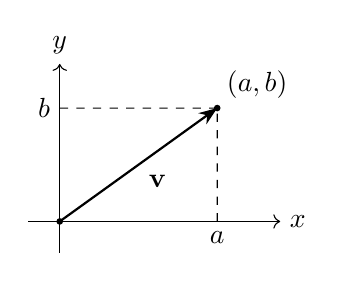
\begin{tikzpicture}[scale=0.8]
    % Axes
    \draw[axis] (-0.5,0) -- (3.5,0) node[right] {$x$};
    \draw[axis] (0,-0.5) -- (0,2.5) node[above] {$y$};
    % Origin
    \fill (0,0) circle (1.5pt);
    % Point and vector
    \coordinate (P) at (2.5,1.8);
    \fill (P) circle (1.5pt) node[above right] {$(a,b)$};
    \draw[vector] (0,0) -- (P) node[midway, below right] {$\mathbf{v}$};
    % Dashed lines to show coordinates
    \draw[dashed, thin] (2.5,0) -- (P);
    \draw[dashed, thin] (0,1.8) -- (P);
    \node[below] at (2.5,0) {$a$};
    \node[left] at (0,1.8) {$b$};
\end{tikzpicture}

\small\textit{Elements of $\R^2$ can be thought of as points or as vectors.}
\end{center}
\smallskip

\begin{tcolorbox}[colframe=black!50]
\textbf{1.12 Example: $\C^4$}

$\C^4 = \{(z_1, z_2, z_3, z_4) : z_1, z_2, z_3, z_4 \in \C\}$
\end{tcolorbox}

\begin{tcolorbox}
\textbf{1.13 Definition: Addition in $\F^n$}

Addition in $\F^n$ is defined by adding corresponding coordinates:
\[
    (x_1, \ldots, x_n) + (y_1, \ldots, y_n) = (x_1 + y_1, \ldots, x_n + y_n)
\]
\end{tcolorbox}

\begin{example}[Vector Addition]
In $\R^3$:
\[
    (1, 2, 3) + (10, 20, 30) = (1+10, 2+20, 3+30) = \boxed{(11, 22, 33)}
\]
\end{example}

\textbf{Geometric intuition:} In $\R^2$ and $\R^3$, addition corresponds to the parallelogram rule: place the tail of the second vector at the head of the first.

\smallskip
\begin{center}
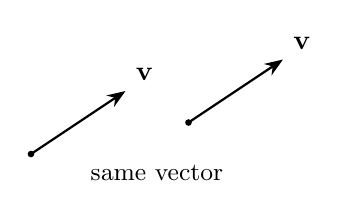
\begin{tikzpicture}[scale=0.8]
    % First vector
    \draw[vector] (0,0) -- (1.5,1) node[above right] {$\mathbf{v}$};
    \fill (0,0) circle (1.5pt);
    % Second vector (same, different position)
    \draw[vector] (2.5,0.5) -- (4,1.5) node[above right] {$\mathbf{v}$};
    \fill (2.5,0.5) circle (1.5pt);
    % Labels
    \node at (2, -0.3) {\small same vector};
\end{tikzpicture}

\small\textit{A vector---same length and direction = same vector.}
\end{center}
\smallskip

\smallskip
\begin{center}
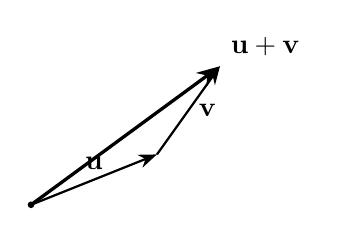
\begin{tikzpicture}[scale=0.8]
    % Origin dot
    \fill (0,0) circle (1.5pt);
    % Vector u
    \draw[vector] (0,0) -- (2,0.8) node[midway, above] {$\mathbf{u}$};
    % Vector v (at tip of u)
    \draw[vector] (2,0.8) -- (3,2.2) node[midway, right] {$\mathbf{v}$};
    % Sum vector u+v (solid for emphasis)
    \draw[vector, line width=1.2pt] (0,0) -- (3,2.2) node[above right] {$\mathbf{u}+\mathbf{v}$};
\end{tikzpicture}

\small\textit{The sum of two vectors (tip-to-tail method).}
\end{center}
\smallskip

\begin{tcolorbox}
\textbf{1.14 Commutativity of Addition in $\F^n$}

If $x, y \in \F^n$, then $x + y = y + x$.
\end{tcolorbox}

\textbf{Proof:} Suppose $x = (x_1, \ldots, x_n)$ and $y = (y_1, \ldots, y_n)$. Then:
\begin{align*}
x + y &= (x_1, \ldots, x_n) + (y_1, \ldots, y_n) \\
      &= (x_1 + y_1, \ldots, x_n + y_n) \\
      &= (y_1 + x_1, \ldots, y_n + x_n) \\
      &= (y_1, \ldots, y_n) + (x_1, \ldots, x_n) \\
      &= y + x
\end{align*}
where the third equality uses commutativity of addition in $\F$. \hfill $\square$

\begin{tcolorbox}
\textbf{1.15 Notation: $0$}

Let $0$ denote the list of length $n$ whose coordinates are all $0$:
\[
    0 = (0, \ldots, 0)
\]
\end{tcolorbox}

\textbf{Geometric intuition:} The zero vector $0$ represents the origin. Adding $0$ to any vector leaves it unchanged---you're adding ``no displacement.''

\begin{tcolorbox}[colframe=black!50]
\textbf{1.16 Example: The Zero Vector Notation}

When we write $x + 0 = x$ for $x \in \F^n$, the symbol $0$ means the \textbf{zero vector}:
\[
    0 = (0, 0, \ldots, 0) \quad \text{($n$ zeros)}
\]

\textbf{Why?} Addition in $\F^n$ is only defined for two vectors. Since $x$ is a vector, the $0$ in ``$x + 0$'' must also be a vector---not the number zero.

\textbf{Example in $\R^3$:}
\[
    (1, 2, 3) + 0 = (1, 2, 3) + (0, 0, 0) = (1, 2, 3) \checkmark
\]

\textbf{Key point:} The symbol ``$0$'' means different things depending on context:
\begin{itemize}
    \item In $\F$ (scalars): $0$ is the number zero
    \item In $\F^n$ (vectors): $0$ is the zero vector $(0, \ldots, 0)$
\end{itemize}
\end{tcolorbox}

\begin{tcolorbox}
\textbf{1.17 Definition: Additive Inverse in $\F^n$}

For $x \in \F^n$, the \textbf{additive inverse} of $x$, denoted $-x$, is the vector $-x \in \F^n$ such that $x + (-x) = 0$.

If $x = (x_1, \ldots, x_n)$, then $-x = (-x_1, \ldots, -x_n)$.
\end{tcolorbox}

\textbf{Note:} Subtraction is defined by $x - y = x + (-y)$.

\textbf{Geometric intuition:} In $\R^2$, $-x$ is the vector with the same length as $x$ but pointing in the opposite direction.

\smallskip
\begin{center}
\begin{tikzpicture}[scale=0.8]
    % Origin dot
    \fill (0,0) circle (1.5pt);
    % Vector x
    \draw[vector] (0,0) -- (2,0.8) node[above right] {$\mathbf{x}$};
    % Vector -x
    \draw[vector] (0,0) -- (-2,-0.8) node[below left] {$-\mathbf{x}$};
\end{tikzpicture}

\small\textit{A vector and its additive inverse.}
\end{center}
\smallskip

\textbf{Why not coordinate-wise multiplication?} We \textit{could} define multiplication of two vectors by multiplying corresponding coordinates, but this is not useful for linear algebra. Instead, \textbf{scalar multiplication} (multiplying a vector by a number) is central to our subject.

\begin{tcolorbox}
\textbf{1.18 Definition: Scalar Multiplication in $\F^n$}

The product of a number $\lambda \in \F$ and a vector in $\F^n$ is computed by multiplying each coordinate by $\lambda$:
\[
    \lambda(x_1, \ldots, x_n) = (\lambda x_1, \ldots, \lambda x_n)
\]
\end{tcolorbox}

\begin{example}[Scalar Multiplication in $\R^n$]
Here $\lambda = -2 \in \R$.
\[
    -2(1, 2, 3) = (-2 \cdot 1, -2 \cdot 2, -2 \cdot 3) = \boxed{(-2, -4, -6)}
\]
\end{example}

\begin{example}[Scalar Multiplication in $\C^n$]
Here $\lambda = 1+i \in \C$.
\begin{align*}
    (1+i)(2, -i) &= ((1+i) \cdot 2, (1+i)(-i)) \\
    &= (2 + 2i, -i - i^2) \\
    &= (2 + 2i, -i + 1) \\
    &= \boxed{(2+2i, 1-i)}
\end{align*}
\end{example}

\textbf{Geometric intuition in $\R^2$:}
\begin{itemize}
    \item If $\lambda > 0$: $\lambda x$ points in the same direction as $x$, with length $\lambda$ times the length of $x$.
    \item If $\lambda > 1$: stretches (longer). If $0 < \lambda < 1$: shrinks (shorter).
    \item If $\lambda < 0$: $\lambda x$ points in the opposite direction, with length $|\lambda|$ times the length of $x$.
\end{itemize}

\begin{tcolorbox}[colframe=black!50]
\textbf{Direction Preservation Property}

All scalar multiples of a nonzero vector $x$ lie on a single line through the origin.

\textbf{Proof:} Let $x = (x_1, \ldots, x_n) \neq 0$. The set of all scalar multiples is:
\[
    \{\lambda x : \lambda \in \F\} = \{(\lambda x_1, \ldots, \lambda x_n) : \lambda \in \F\}
\]
This is precisely the parametric equation of the line through the origin with direction vector $x$. As $\lambda$ varies over $\F$, we trace out every point on this line. \qed

\textbf{Key insight:} This property is fundamental to linear maps (Chapter 3)---they preserve these lines through the origin.
\end{tcolorbox}

\smallskip
\begin{center}
\begin{tikzpicture}[scale=0.8]
    % Vertical alignment line (dashed)
    \draw[dashed, thin, gray] (0,0.3) -- (0,-2.7);
    % Base vector x
    \draw[vector] (0,0) -- (2,0) node[above right] {$\mathbf{x}$};
    % Half x
    \draw[vector] (0,-1.2) -- (1,-1.2) node[above right] {$\frac{1}{2}\mathbf{x}$};
    % -3/2 x
    \draw[vector] (0,-2.4) -- (-3,-2.4) node[above left] {$-\frac{3}{2}\mathbf{x}$};
    % Origin marks
    \fill (0,0) circle (1.5pt);
    \fill (0,-1.2) circle (1.5pt);
    \fill (0,-2.4) circle (1.5pt);
\end{tikzpicture}

\small\textit{Scalar multiplication: scaling and reversing vectors.}
\end{center}
\smallskip

\begin{result}
\textbf{Scalar multiplication vs dot product:} Scalar multiplication takes a scalar and a vector, producing a \textbf{vector}. The dot product (Chapter 6) takes two vectors and produces a \textbf{scalar}. These are different operations.

\textbf{Generalization:} The dot product in $\R^n$ generalizes to the \textbf{inner product} in Chapter 6, which works for both $\R^n$ and $\C^n$ (and more abstract vector spaces).
\end{result}

%==============================================================================
\section{Digression on Fields}
%==============================================================================

A \textbf{field} is a set containing at least two distinct elements called $0$ and $1$, along with operations of addition and multiplication satisfying all properties listed in 1.3.

\begin{itemize}
    \item $\R$ and $\C$ are fields.
    \item The set of rational numbers $\mathbb{Q}$ is a field.
    \item The set $\{0, 1\}$ with usual addition and multiplication (except $1 + 1 = 0$) is a field.
\end{itemize}

\textbf{Note:} This book deals only with $\R$ and $\C$. However, many definitions, theorems, and proofs work for arbitrary fields. If you prefer, think of $\F$ as denoting an arbitrary field (except in Chapters 6--7 on inner products, where $\F = \C$ is sometimes required).

%==============================================================================

\newpage
%==============================================================================
\section*{Key Takeaways}
%==============================================================================

\begin{enumerate}
    \item \textbf{Complex numbers extend the reals:} $\C = \{a + bi : a, b \in \R\}$ with $i^2 = -1$
    \item \textbf{$\F^n$ generalizes familiar spaces:} Lists of $n$ scalars with coordinate-wise operations
    \item \textbf{Addition and scalar multiplication:} The two fundamental operations, defined component-wise
    \item \textbf{The zero vector:} $0 = (0, \ldots, 0)$ is the additive identity in $\F^n$
    \item \textbf{Conjugate trick:} Multiply by $\overline{z}/\overline{z}$ to compute complex division
\end{enumerate}

\subsection*{Relevant Exercises}
Practice these problems from LADR to reinforce the material:
\begin{itemize}
    \item Section 1A: 1, 2, 3, 4, 5, 6, 7, 8, 9, 10, 11, 12, 13, 14
\end{itemize}

%==============================================================================
\section*{Exercise Reference}
%==============================================================================

\subsection*{Key Formulas}

\begin{tcolorbox}
\textbf{Complex Inverse:}
\[
    \frac{1}{a+bi} = \frac{a-bi}{a^2+b^2}
\]

\textbf{Addition in $\C$:} $(a+bi) + (c+di) = (a+c) + (b+d)i$

\textbf{Multiplication in $\C$:} $(a+bi)(c+di) = (ac-bd) + (ad+bc)i$

\textbf{Addition in $\F^n$:} $(x_1,\ldots,x_n) + (y_1,\ldots,y_n) = (x_1+y_1,\ldots,x_n+y_n)$

\textbf{Scalar Multiplication:} $\lambda(x_1,\ldots,x_n) = (\lambda x_1,\ldots,\lambda x_n)$
\end{tcolorbox}

\subsection*{Common Problem Types}

\begin{tcolorbox}
\begin{description}[style=nextline, leftmargin=1em, labelindent=0pt]
    \item[Computing Complex Inverses/Roots]
    Multiply numerator and denominator by the conjugate. To verify a root, substitute and compute the power directly.

    \item[Proving Field Properties in $\C$]
    Write complex numbers as $\alpha = a+bi$, $\beta = c+di$. Expand both sides using definitions; compare real and imaginary parts.

    \item[Proving Uniqueness (of inverses, identities)]
    Assume two objects satisfy the defining property. Use that property to show they must be equal.

    \item[Solving Vector Equations]
    Isolate the unknown using additive inverses and scalar multiplication. Work component-wise.

    \item[Showing No Scalar $\lambda$ Exists]
    If $\lambda x = y$, then each component ratio $y_j/x_j$ must equal $\lambda$. Check if all ratios are consistent.

    \item[Proving $\F^n$ Properties]
    Write vectors as $x = (x_1,\ldots,x_n)$. Apply definitions of addition/scalar multiplication, then use field axioms on each component.
\end{description}
\end{tcolorbox}

\end{document}
